\chapter{线性代数 - 线性变换}

\begin{figure}[ht]
  \centering
  
\includegraphics[width=1\linewidth]{asset/茶桁的AI秘籍_Math_18.png}
\end{figure}

\newpage

经历了几节线性代数课程之后, 终于咱们到了最后一节课了。本节课的内容说多不多, 说少也不少。

我们先是要理解一下线性空间和线性变换, 并且探讨一下线性变换的几何意义。然后咱们要去看看特征值和特征向量, 最后, 会使用NumPy来做一次矩阵操作。

好, 让我们开始吧。

\section{线性空间}

之前我说到, 这节课内容说多不多, 说少不少。为什么呢?看似这节课的概念很多, 但是其实都非常简单。就像这一部分, 「线性空间」,  看上去很复杂的样子, 其实内容特别的简单。就相当于在一个新的地方给你说了一下加法和乘法运算。对, 就是就是这么简单。我们要理解的仅仅是概念而已。

可是, 为什么会有这么复杂的东西?因为数学是一个非常严谨的东西, 如果我们要考虑到它内在的一些完备性, 那我们必须用词非常严谨, 把所有该说的话全部说出来, 所以就显得很啰嗦。

但是我们人类对于理解这样的数学定理其实是是有自己的一套体系的, 我们是把它和一些我们已经学到过的知识
去做一个类比, 而在这里类比就是我们这些实数里面的四则运算: 加减乘除, 而这里只用到了加以及乘。


我们先来看一遍, 大家有个了解: 

设$V$是一个非空集合, $P$是一个域, 若: 

\begin{enumerate}
  \item 在V中定义一种运算——加法, 使得V中任意两个元素$\alpha$与 $\beta$ 都依据某一法则 对应于V内唯一确定的一个元素$\alpha$ + $\beta$ , 称为$\alpha$与 $\beta$ 的和;
  \item 在P与V的元素间定义了一种运算, 称为数量乘法, 即对V中任意元素$\alpha$与P中任意元素k, 都按某一法则对应V内唯一确定的一个元素 k$\alpha$, 称为k与$\alpha$的积;
  \item 若上述加法与数量乘法满足以下条件: 
  \begin{enumerate}
   \item $\alpha+\beta=\beta+\alpha$, $\forall\alpha$, $\beta\in V$; 
   \item $\alpha+(\beta+\gamma) = (\alpha+\beta)+\gamma$, $\forall\alpha$, $\beta$, $\gamma\in V$ 
   \item $\exists$ 零元 0 $\in V$, $s.t.$ $\forall\alpha\in V$, 有$\alpha+0 = \alpha$ ;
   \item $\forall\alpha\in V$, $\exists\beta$使$\alpha+\beta = 0$, 记 $\beta = \mbox{-}\alpha$
   \item 对$P$中单位元1, $\forall\alpha\in V$, 有$1\alpha = \alpha$ ;
   \item $\forall k$,  $l\in P$, $\forall\alpha\in V$ , 有$(kl)\alpha =  k(l\alpha)$ 
   \item $\forall k$,  $l\in P$, $\forall\alpha\in V$ , 有$(k+ l)\alpha =  k\alpha+ l\alpha$ ; 
   \item $\forall k\in P$, $\forall\alpha$, $\beta\in V$, 有 $k(\alpha+\beta) =  k\alpha+ k\beta$ 
  \end{enumerate}
\end{enumerate}

则称$V$为域$P$上的一个线性空间, 或向量空间

以上, 我们设$V$是一个非空集合, 就说它里面不是一个东西都没有。然后$P$是一个域, 域代表一个数域,在这里大家也可以理解成某种数的集合就行了。

第一条在$V$里面定义了一种运算加法,使得$V$中任意两个元素$\alpha$, $\beta$根据某一个法则它都对应于V内唯一确定的一个元素$\alpha+\beta$。看上去不就是跟废话一样吗?其实它就是相当于在一个新的领域给你重新定义了一下加法, 不是说与生俱来的。就是我们四则运算里面那个加法, 意义上面差不太多。也许它这里面的加法不是说简单的$1+2=3$, 它也许是比较复杂的, 但是你可以把它理解成加法。比如说向量, 两个向量之间的加法。它就是对应位置相加, 就和我们数的相加就有点不一样了。

第二点就定义了一个数量乘法, 一个数k乘上一个向量$\alpha$, 就称为$k$与$\alpha$的一个积, 就这么一个东西。

第三点有8条性质, 但这8条非常简单, 就跟咱们数的那些结合率、交换率一模一样。比如第七条, $(k+ l)\alpha =  k\alpha+ l\alpha$, 单独一眼望上去: “哇这么多内容我不想看了”, 但你定睛一看: 我靠, 这么简单, 这是小学上过的内容, 结合率、分配率这些东西。

所以在这里大家就知道这么一个回事就行了, 我就不一一的对给大家去说了。就是说满足这三条的东西, $V$就构成的一种线性空间, 叫做向量空间。并且这些性质可以类比四则运算, 就这么一回事。没什么太多可说的了, 简单的理解, 线性空间, 就是由向量构成的一些空间。

如果哪一天你忘记具体要满足哪些条件, 你再去查, 平时的时候你不需要去查。

那这么简单为什么我们还要单独拿出来说它呢?那是因为, 我们接下来要说的线性变换是定义在线性空间上面的。

\section{线性变换}

线性空间$V$上的一个变换$\mathcal{A}$称为线性变换, 若对于$V$中任意元素$\alpha$,$\beta$和数域$P$中任意$k$, 都有: 

\begin{align*}
  \mathcal{A}(\alpha+\beta) & = \mathcal{A}(\alpha) + \mathcal{A}(\beta) \\
  \mathcal{A}( k\alpha) & =  k\mathcal{A}(\alpha)
\end{align*}

注意, 这里我用的是一个花体的一个拉丁文字符$\mathcal{A}$, 严格意义上面来说线性变换都得用花体来表示。

当它满足什么样的条件的时候, 就是向量在向量空间里面任意的两个向量$\alpha$和$\beta$, 以及数据$P$里面的任意一个数$k$它都满足以上两个式子, 第一个式子中的结合率, 以及第2条$\mathcal{A}$对$k\alpha$作用等于k提取出来$\mathcal{A}$对$\alpha$法作用。

如果满足这两个的话, 变换$\mathcal{A}$它就被称为线性变换。

数学上面的一个比较生硬的定义, 大家可能也联想不到什么东西, 那其实实质上, 符合上述定义的每一个方阵都代表着一种线性变换。

也就是, 变换其实可以用一个矩阵来表示, 比如说我们前面有讲过一个线性方程组的一个式子: $Ax = B$, 如果不太记得的, 可以回头再去看看我们第一节的线性代数的课程。其实在那里就相当于A对x去做了一个变换, 把它变成了B。

这里A叫做线性变换, 大家也可以理解成一个函数, 就像$f(x)=y$一样, $A$就通过它自己的向量乘法把$x$给它变成了$B$, 所以这就是线性变换的一个本质。

0变换对应的矩阵是什么?我们已经说过,其实每一个矩阵只要符合定义都代表着一种线性变换, 所以以后我们说到线性变换都直接用矩阵的形式来表示。这里我们来考虑一下零变化它是否是一个线性变化。

这里举一个例子: 

例: 试判断零变换是否为线性变换?

解: 不失一般性, 考虑二阶的情况

\begin{align*}
  & A = \begin{bmatrix} 0 & 0 \\ 0 & 0 \end{bmatrix}, \alpha,\beta \in R^2,  \alpha=\begin{bmatrix}  x \\ y\end{bmatrix} , \beta = \begin{bmatrix} r \\ t\end{bmatrix} \\
  & A(\alpha+\beta) = \begin{bmatrix} 0&0\\0&0\end{bmatrix}\begin{bmatrix} x+r \\ y+t \end{bmatrix} = \begin{bmatrix} 0 \\ 0 \end{bmatrix} \\
  & A\alpha+A\beta = \begin{bmatrix} 0&0\\0&0\end{bmatrix}\begin{bmatrix} x \\ y \end{bmatrix} + \begin{bmatrix} 0&0\\0&0\end{bmatrix}\begin{bmatrix} r \\ t \end{bmatrix}  = \begin{bmatrix} 0 \\ 0 \end{bmatrix} \\
  & A(k\alpha) = \begin{bmatrix} 0 & 0 \\ 0 & 0\end{bmatrix}\begin{bmatrix}kx \\ ky \end{bmatrix} = \begin{bmatrix} 0 \\ 0 \end{bmatrix}, \\
  & kA\alpha = k\begin{bmatrix} 0 & 0 \\ 0 & 0\end{bmatrix}\begin{bmatrix}x \\ y \end{bmatrix} = \begin{bmatrix} 0 \\ 0 \end{bmatrix}\\
  & A(\alpha+\beta) = A\alpha + A\beta, A(k\alpha) = kA\alpha \\
  &  \mbox{零变换是线性变换}
\end{align*}

不失一般性, 我们就来看一下二阶的这么一个情况。比如$A$是一个0矩阵,全部都为0。然后$\alpha$,$\beta$是一个二维的向量。然后我们来看一下当$A$作用于$\alpha+\beta$的时候计算结果是$[0,0]$。

然后$A\alpha+A\beta$, 分别相乘做向量乘法, 再加在一起。依然得到的是$[0, 0]$。所以我们发现和是相等的, 那同理其实很简单, 我们能证明$A(k\alpha)$和$kA\alpha$也是相等的, 所以满足这些条件。

那么我们就知道, 零变换它是一种线性变换。

在神经网络里面, 某一层的数据经过权重矩阵, 相乘了之后传到下一层, 其实就是相当于做了一个线性变换。那我们知道, 单纯的线性变换并不能帮我们解决很多问题, 所以引入了激活函数。引入激活函数就是引入了一种非线性变换, 这就是线性变换和神经网络的联系。

那线性变换对于向量具体有哪些比较直观的意义?

\section{线性变换的几何意义}

我们来看一个之前曾经看到过的例子, 这个例子我们在导论课 \hyperlink{3.线性代数基础}{《3. 数学导论 - 线性代数基础(矩阵)》}里面提到过。有一个矩阵, 再有一个向量, 让它们做一个矩阵乘法。

来看一下计算: 

\begin{align*}
  & \begin{bmatrix}
  cos90^{\circ} & -sin90^{\circ} \\
  sin90^{\circ} & cos90^{\circ}
  \end{bmatrix}
  \begin{bmatrix}
  2 \\ -2
  \end{bmatrix} 
  = \begin{bmatrix}
  2cos90^{\circ} + 2sin90^{\circ} \\
  2sin90^{\circ} - 2cos90^{\circ}
  \end{bmatrix} 
  = \begin{bmatrix} 2 \\ 2 \end{bmatrix}
\end{align*}

通过矩阵乘法的计算, 能得到三角函数的矩阵把我们原来的向量 $[2 -2]$ 变成了向量 $[2 2]$。在这里, 矩阵起到的作用就是将一个向量旋转了$90^{\circ}$, 如图\ref{fig:img19_1}: 

\begin{figure}[ht]
  \centering
  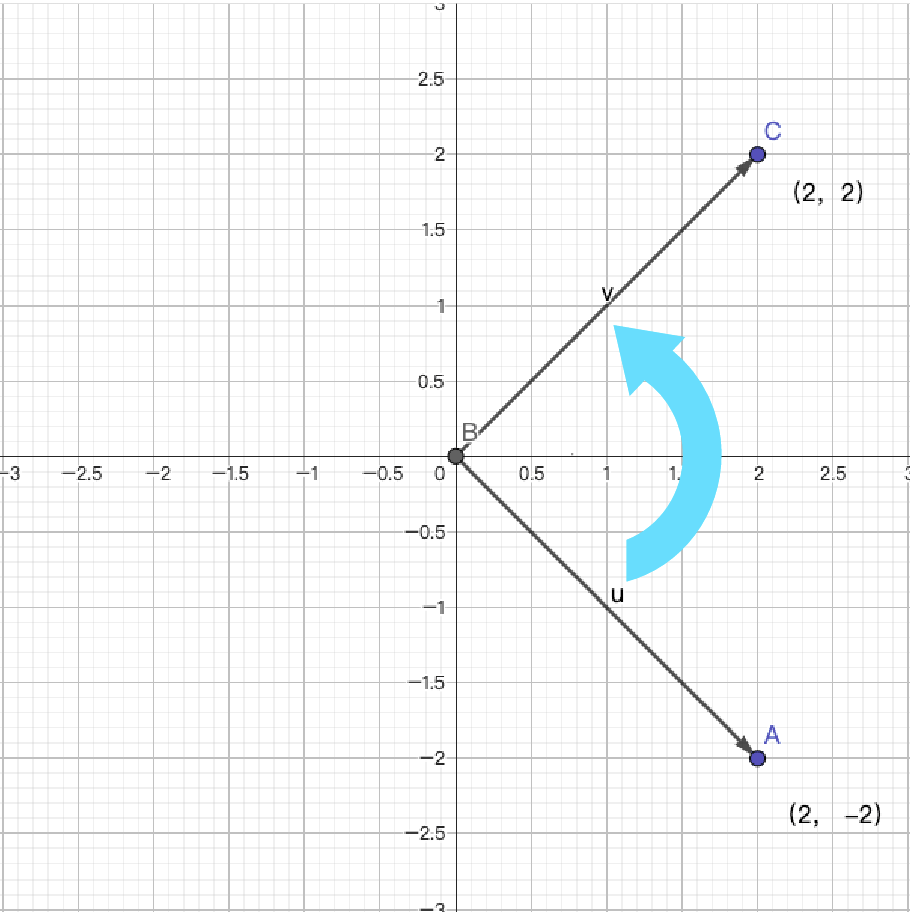
\includegraphics[width=0.5\linewidth]{asset/20230913133039.png}
  \caption{}
  \label{fig:img19_1}
\end{figure}


我们再看一个例子: 

\begin{align*}
& \begin{bmatrix}
2 & 0 \\
0 & 1
\end{bmatrix}
\begin{bmatrix}
2 \\ -2
\end{bmatrix} = \begin{bmatrix}
2 \times 2 + 0 \times (-2) \\
0 \times 2 + 1 \times (-2)
\end{bmatrix} = \begin{bmatrix} 4 \\ -2 \end{bmatrix}
\end{align*}

经过矩阵乘法之后,我们发现它将向量$[2 -2]$变成了$[4 -2]$, 这相当于把向量沿x方向上拉升为了原来的两倍, 原来是2现在是4, y方向上有没有变化, 如图\ref{fig:img19_2}: 

\begin{figure}[ht]
  \centering
  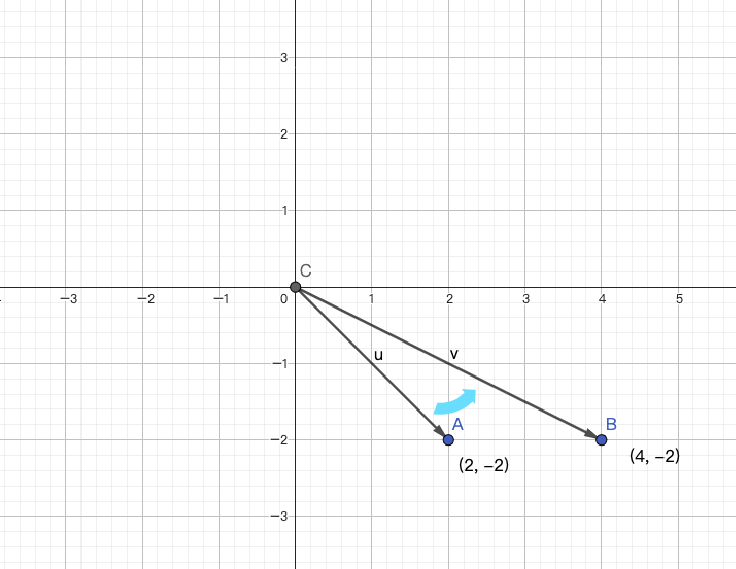
\includegraphics[width=0.5\linewidth]{asset/20230913135453.png}
  \caption{}
  \label{fig:img19_2}
\end{figure}

我们观察一下矩阵, 其实很容易发现, 矩阵内主对角线上的2实际作用于向量里的2,  而矩阵主对角线上的1, 实际作用的是向量里的-2, 看一下计算过程就知道了。

因为长度没有发生变化, 所以y方向上保持不变。而x方向上它拉伸了两倍, 所以线性变换除了旋转之外, 它还可以让项链产生一个拉伸的效果。

\section{特征值与特征向量}

很快, 我们就来到了线性代数课程里的最后一部分, 就是特征与特征向量。这个在我们整个线性代数也是非常重要的一个部分, 包括很多机器学习的方法, 比如说PCA降维。它其实核心也是用到了特征值概念。

什么叫特征值和特征向量, 就对于n阶的方阵A, 若有数$\lambda$ 以及非零n维向量$x$使得: $Ax = \lambda x$

在这种情况下, 我们就把数$\lambda$ 称为矩阵A的一个特征值。满足式子的一个$x$称为矩阵$A$关于$x$关于$\lambda$ 的一个特征向量。

式子的含义就是, $A$矩阵对$x$向量去做一个线性变换, 效果是在$x$原来的方向上拉伸或者压缩了$\lambda$ 倍。方向并没有变化, 只是沿着原来的方向伸缩了$\lambda$ 倍。这也正是其几何意义。

我们再进一步, 对特征值和特征向量去做一个变换。

设$A$为n阶方阵, 则 $Ax = \lambda x \to (A - \mbox{−} \lambda I)x = \vec 0$

$Ax = \lambda x$, 式子两边相等, 那我把右边给它减到左边。但是因为这里$A$是一个n阶的方阵, $\lambda$ 是一个数, 不能让$A$直接减去$\lambda$ , 因为它俩就不能做运算, 一个是矩阵一个是数。所以在这里我们可以把$\lambda$ 乘以$I$, 就可以将$\lambda x$ 变成$\lambda Ix$ 。$I$就是一个单位矩阵。

这个时候$A$是n阶的, $\lambda$ 也是一个n阶的, 就可以做减法了。所以这里也是一个比较困难的地方, 而且在这里$\lambda$ 和$x$之间加入一个$I$单位矩阵, 是不影响结果的。$\lambda Ix$ 等于$\lambda x$ , 因为$Ix$等于$x$, 所以是可以成立的。

然后就等于$\vec 0$,  这里0上面有一个箭头表示不是数字0, 而是一个向量0。

然后我们有没有惊讶的发现, 不是很像$Ax = B$的形式吗? 这里$B$等于0,那它不就是一个齐次线性方程组吗?它有n个未知量以及n个方程的一个齐次线性方程组。

我们来回忆一下, \textbf{对于一个齐次线性方程组,  它有非零解的充要条件是系数行列式为0: $|A - \lambda I| = 0$}。这个是我们在 \hyperlink{15.线性代数}{《15. 线性代数 - 克拉默法则》}里面说过的, 大家可以再翻回去看一下。

就是说, 如果系数行列式不为0的话, 那它的解为1。我们可以用克拉默法则, $\frac{|A_i|}{|A|}$去做, 它只有0解。

也就是说x必须也是0向量, 如果这里有非0解的话。就是$x$不是0向量的这么一个解的话, 那就只能让克拉莫法则失效。怎么样让它失效?系数行列式为0。

所以系数行列式$|A - \lambda I|$等于0, 同时$|A - \lambda I|$也被称为$A$的一个特征多项式。

我们通过求解$|A - \lambda I|=0$这个式子得到A的特征值, 因为里面A的系数都是已知的, I里面只有对角线是1, 其它都是0, 只有$\lambda$ 的值是需要我们去求解的, 所以这里是关于$\lambda$ 的一个方程。我们通过解方程可以得到$\lambda$ 的值, 就是线性变换或者说A的一个特征值。

特征值求出来之后, 将求得的特征值代入$Ax = \lambda x \to (A - \lambda I)x = \vec 0$ 中求得对应的特征向量。

我们分了两步: 第一步求出了A的特征值, 第二步求出来相应的特征向量。

说概念大家肯定也会觉得很无聊, 还会又些晕乎乎的, 我们来举一个例子: 

例子: 求下列矩阵的特征值和特征向量: 

\begin{align*}
  A = \begin{bmatrix}2 & 1 \\ 3 & 0 \end{bmatrix}
\end{align*}

一个$2 \times 2$的二阶的一个方阵, 然后我们来尝试求矩阵的特征值和特征向量。

首先我们来看一下它的特征方程是什么: 

\begin{align*}
  |\lambda I-A| & = \begin{bmatrix} \lambda -2 & -1 \\ -3 & \lambda  \end{bmatrix} \\
  & = \lambda ^2 - 2\lambda  -3 = 0 \\
  & \lambda _1 = -1, \lambda _2 = 3
\end{align*}

$\lambda I-A$, 有的同学可能会注意到之前是$A-\lambda I$, 这里呢又变成$\lambda I-A$。其实无所谓, 都可以。之前我们是将等式$Ax = \lambda x$右边移动到左边编程$(A - \lambda I)x$, 现在是将等式左边移动到右边, 其实是等价的。

$\lambda I-A$是它的一个特征多项式, 写出来就是主对角线上全部都是$\lambda$ , 其他位置都是0的一个二阶矩阵。再之后, 矩阵的减法, 减出来之后, 行列上的做法, 二阶的非常简单, 主对角线元素相乘减去负对角线上面的元素, 化成多项式$\lambda ^2 - 2\lambda  -3 = 0$。

通过解特征方程, 这里其实也就是我们之前提到的$|A - \lambda I| =0$。

为什么要令它等于0, 只有它系数行列式等于0, 我齐次线性方式组才有非0解。

最后求出来有两个特征值, 一个是-1一个是3。那接着, 我们就要根据两个解来分布讨论, 来分别代入进去求解特征向量: 

当$\lambda 1 = -1$时, 方程组$(A - \lambda I)x = \vec 0$解有: 

\begin{align*}
\begin{cases}
-3x - y = 0 \\
-3x - y = 0
\end{cases}
\to\mbox{一个特征向量}a_1 = \begin{bmatrix} 1 \\ -3 \end{bmatrix}
\end{align*}

当$\lambda 2 = 3$时, 方程组$(A - \lambda I)x = \vec 0$解为: 

\begin{align*}
\begin{cases}
x - y = 0 \\
-3x + y = 0
\end{cases}
\to \mbox{一个特征向量} a_2 = \begin{bmatrix} 1 \\ 1 \end{bmatrix}
\end{align*}

注意: \textbf{这里有个措辞叫做「一个特征向量」}。

为什么说是「一个」, 而不是说「特征向量」为$a_1$。因为$a_1$乘上任意一个实数倍它都是方程组的解。大家可以看一下, 其实方程组它得到的结果这两个式子是一样的, $y=3x$, 只要令第2个数是第1个数$-3$倍就行了。所以特征善量可以是$[1, -3]$也可以是$[2, -6]$, 有无穷多个。这里措辞大家千万要注意, 叫做「一个」。

通过步骤我们就把一个矩阵的特征值和他的特征向量给他求出来了。

对于更复杂一点的矩阵, 其实它的解法也是一样的。核心思想就是这些, 能把例子看懂了就OK了。

好, 接下来, 咱们来看看再NumPy库里, 关于矩阵操作的一些内容。

\section{NumPy的矩阵操作}

我们先引入NumPy库: 

\begin{python}
import numpy as np    # 导入NumPy模块
print(np.version.version)   # 查看当前安装的NumPy的版本

---
1.23.3
\end{python}

不知道有多少同学之前看过我的Python基础课程, 看过的小伙伴, 还记得NumPy的基本数据结构吗?让我们先来回忆一下NumPy的基本数据结构和对数组的操作: 

\begin{python}
a = np.array([[1, 2, 3], [4, 5, 6]])   # NumPy中基本数据类型-数组的声明
print(a)

---
[[1 2 3]
 [4 5 6]]
\end{python}

数组的维度

\begin{python}
print("数组a的维度个数为: ", a.ndim)  # 数组的维度

---
数组a的维度个数为:  2
\end{python}

数组各个维度的长度

\begin{python}
print("数组a的各个维度长度为: ", a.shape)  # 数组各个维度的长度

---
数组a的各个维度长度为:  (2, 3)
\end{python}

数组里元素总数

\begin{python}
print("数组a中元素总数为: ", a.size)  # 数组里元素总数

---
数组a中元素总数为:  6
\end{python}

数组元素的类型

\begin{python}
print("数组a中元素类型为: ", a.dtype)  # 数组元素的类型

---
数组a中元素类型为:  int64
\end{python}

用arange函数创建数组 (开始值, 终值, 步长)

\begin{python}
b = np.arange(0, 20, 5)     # 用arange函数创建数组 (开始值, 终值, 步长)
print(b)

---
[ 0  5 10 15]
\end{python}

改变数组的形状

\begin{python}
b.reshape(2, 2)         # 改变数组的形状

---
array([[ 0,  5],
       [10, 15]])
\end{python}

用linspace函数创建数组(开始值, 终值, 元素个数)

\begin{python}
c = np.linspace(0, 2, 10)   # 用linspace函数创建数组(开始值, 终值, 元素个数)
print(c)

---
[0.         0.22222222 0.44444444 0.66666667 0.88888889 1.11111111
 1.33333333 1.55555556 1.77777778 2.        ]
\end{python}

快速创建元素全为0的数组

\begin{python}
zero_arr = np.zeros((3,4))   # 快速创建元素全为0的数组
print(zero_arr)

---
[[0. 0. 0. 0.]
 [0. 0. 0. 0.]
 [0. 0. 0. 0.]]
\end{python}

快速创建元素全为1的数组, 并将类型设置为整型

\begin{python}
one_arr = np.ones((2,3,4), dtype=np.int64)   # 快速创建元素全为1的数组, 并将类型设置为整型
print(one_arr)

---
[[[1 1 1 1]
  [1 1 1 1]
  [1 1 1 1]]

 [[1 1 1 1]
  [1 1 1 1]
  [1 1 1 1]]]
\end{python}

快速创建对角阵 

\begin{python}
eye_arr = np.eye(3)   # 快速创建对角阵 
print(eye_arr)

---
[[1. 0. 0.]
 [0. 1. 0.]
 [0. 0. 1.]]
\end{python}

\begin{python}
arr = np.array([1, 2, 3, 4, 5, 6])
print(arr[0:4])      
print(arr[0:4:2])

---
[1 2 3 4]
[1 3]
\end{python}

对数组中每个元素的遍历

\begin{python}
for ele in arr:     # 对数组中每个元素的遍历
    print(ele)
    
---
1
2
3
4
5
6
\end{python}

更改arr数组的形状

\begin{python}
arr = arr.reshape(2,3)     # 更改arr数组的形状
print(arr)

---
[[1 2 3]
 [4 5 6]]
\end{python}

在arr数组里选择第一维度的第一个子序列, 

\begin{python}
print(arr[0,:])            # 在arr数组里选择第一维度的第一个子序列, 

---
[1 2 3]
\end{python}

在arr数组里选择第一维度的第一个子序列里的第一个元素

\begin{python}
print(arr[0, 0])           # 在arr数组里选择第一维度的第一个子序列里的第一个元素

---
1
\end{python}

在arr数组里选择第二维度的第二个子序列里的所有元素

\begin{python}
print(arr[:, 1])           # 在arr数组里选择第二维度的第二个子序列里的所有元素

---
[2 5]
\end{python}

声明两个二维数组

\begin{python}
arr1 = np.array([[1, 2], [3, 4]])     # 声明两个二维数组
print(arr1)
print("********")
arr2 = np.array([[5, 6], [7, 8]])
print(arr2)

---
[[1 2]
 [3 4]]
********
[[5 6]
 [7 8]]
\end{python}

两个数组元素级别的差运算

\begin{python}
print(arr2-arr1)     # 两个数组元素级别的差运算

---
[[4 4]
 [4 4]]
\end{python}

两个数组元素级别的和运算

\begin{python}
print(arr2+arr1)     # 两个数组元素级别的和运算

---
[[ 6  8]
 [10 12]]
\end{python}

两个数组元素级别的乘运算

\begin{python}
print(arr2*arr1)     # 两个数组元素级别的乘运算

---
[[ 5 12]
 [21 32]]
\end{python}

两个数组元素级别的除运算

\begin{python}
print(arr2/arr1)     # 两个数组元素级别的除运算

---
[[5.         3.        ]
 [2.33333333 2.        ]]
\end{python}

数组元素级别的乘方运算 

\begin{python}
print(arr1**2)     # 数组元素级别的乘方运算 

---
[[ 1  4]
 [ 9 16]]
\end{python}

两个数组之间的矩阵乘积运算

\begin{python}
print(arr1@arr2)     # 两个数组之间的矩阵乘积运算

---
[[19 22]
 [43 50]]
\end{python}

使用dot进行的两个数组之间的矩阵乘积运算

\begin{python}
print(np.dot(arr1, arr2))   # 使用dot进行的两个数组之间的矩阵乘积运算
print("*" * 10)
print(arr1.dot(arr2))

---
[[19 22]
 [43 50]]
**********
[[19 22]
 [43 50]]
\end{python}

数组的转置

\begin{python}
print(arr1.T)      # 数组的转置

---
[[1 3]
 [2 4]]
\end{python}

数组中最大元素, 以及沿第一位度和第二维度值最大元素的索引。

\begin{python}
arr3 = np.array([[1, 2, 3], [4, 5, 6]])
print(arr3)
print("arr1中最大元素的索引为: ", np.argmax(arr3))                    # 数组中值最大元素的索引
print("arr1中沿第一个轴最大元素的索引为: ", np.argmax(arr3, axis=0))    # 数组中沿第一个维度值最大元素的索引
print("arr1中沿第二个轴最大元素的索引为: ", np.argmax(arr3, axis=1))    # 数组中沿第二个维度值最大元素的索引

---
[[1 2 3]
 [4 5 6]]
arr1中最大元素的索引为:  5
arr1中沿第一个轴最大元素的索引为:  [1 1 1]
arr1中沿第二个轴最大元素的索引为:  [2 2]
\end{python}

NumPy中array与matrix的异同

\begin{python}
# NumPy中array与matrix的异同
import numpy as np
a_arr = np.array([1,2])
print("Array形式的a形状为: ", a_arr.shape)
a_mat = np.mat([1,2])
print("Matrix形式的a形状为: ", a_mat.shape)

---
Array形式的a形状为:  (2,)
Matrix形式的a形状为:  (1, 2)
\end{python}

我们再来看看最常用的矩阵运算, 首先, 是矩阵的转置

\begin{python}
# 得到矩阵的转置
mat_temp = np.mat([[1,2],[3,4]])
print("此矩阵为: \n", mat_temp)
print('*' * 10)
print("此矩阵的转置为: \n", mat_temp.T)

---
此矩阵为: 
 [[1 2]
 [3 4]]
**********
此矩阵的转置为: 
 [[1 3]
 [2 4]]
\end{python}

得到矩阵的逆

\begin{python}
# 得到矩阵的逆
mat_temp = np.mat([[1,2],[3,4]])
print("此矩阵为: \n", mat_temp)
print('*' * 10)
mat_inv = mat_temp.I
print("此矩阵的逆矩阵为: \n", mat_inv)
print("此矩阵与它的逆矩阵相乘得到: \n", np.round(mat_temp.dot(mat_inv)))    # np.round用来保留结果到指定位数
\end{python}

求解系数矩阵决定的线性方程组

\begin{python}
import numpy as np
equa = np.mat([[1,2,3],[4,5,6]])
print("此线性方程组为: \n", equa)
print('*' * 10)
A = np.array([[1,2], [4,5]])   # 2x2系数矩阵
b = np.array([3,6])            # 2x1矩阵
res = np.linalg.solve(A,b)     # 求解该系数矩阵决定的线性方程组
print("此线性方程组的解为: \n", res.reshape(1,2).T)

---
此线性方程组为: 
 [[1 2 3]
 [4 5 6]]
**********
此线性方程组的解为: 
 [[-1.]
 [ 2.]]
\end{python}

除此之外, 我们还可以换一种方式求解: 


\begin{python}
import numpy as np
equa = np.mat([[1,2,3],[4,5,6]])
print("此线性方程组为: \n", equa)
print('*' * 10)
A = np.mat([[1,2], [4,5]])   # 2x2系数矩阵
b = np.mat([3,6]).T  # 2x1矩阵(须为列向量的形式)
res = np.linalg.solve(A,b)   # 求解该系数矩阵决定的线性方程组
print("此线性方程组的解为: \n", res)

---
此线性方程组为: 
 [[1 2 3]
 [4 5 6]]
**********
此线性方程组的解为: 
 [[-1.]
 [ 2.]]
\end{python}

好了, 小伙伴, 随着这节课的结束, 线性代数部分也就到这里结束了。大家下来要多多练习。

下一节课, 我们正式进入「概论与统计」部分。